In the wind tunnel canopy flow model, the turbulence is inhomogeneous in essence. Furthermore, the turbulence levels are very strong with turbulence intensity well over 100\% inside the canopy layer. This means that the flow fluctuates strongly both in space and in time. As a consequence we had to determine optimized values for the limiting change in velocity and acceleration between the frames for each individual run. For this we used a principle of minimizing the change of tracking results, given the change in tracking parameters. In other words, we evaluate a cost function based on the change in tracking results.\alex{it has to start with some objectively defined cost function that means ``better quality'' or ``lower uncertainty'', if i understand correctly the minimum of changes also present when all the parameters are at saturation, i.e. when we track everything we can. what changes then? }  For the conservative, too small, limiting values, the tracking algorithm cannot track nearly any particles and very few trajectories will result. \alex{for whatever value below the real particle velocity, we get zero accuracy as we track only wrong pairs that are not the right ones. for whatever value which is much larger than the real velocity value, e.g. size of the observation volume, we are supposed to choose the right ones as they are within the list of possibilities, but the choice becomes too expensive computationally and also the error percentage grows. we sometimes can choose particles that are not the right ones, using a simple criteria. if we'd have very complex tracking algorithm that can eventually choose the right ones, maybe we won't need to talk about it at all. } As the thresholds are increased, more trajectories can be found, so that the tracking results grow rapidly. \alex{what is ``tracking results'' - you mean the ratio of linked particles to the total number of identified and stereo-matched particles?}
In the opposite case of a very liberal choice of tracking parameters, the algorithm will connect nonphysical trajectories, finding large numbers of false positives. \alex{why? is it the algorithm fault or is it just something wrong with our criteria?} Here too, the algorithm will be able to connect more particles as the threshold is increased. \alex{precisely, so?}
However, in the transition between a too conservative and too liberal parameter settings, there exists a range in which a balance is obtained - sufficient physical trajectories are found, with a minimal number of false positives.\alex{yes, but what does it mean a balance and how do you define false negative and false positive?} In this range of parameters the tracking algorithm searches particles over distances that are smaller than the average distance between particles.\alex{i'm not sure it's true, how do you prove it? why not to start from here - find what is the average distance between particles in the frame - this you know before tracking, set the search region for the maximum possible and use it} The region is characterized by a plateau of the graph of the number of trajectories connected, vs. the tracking parameters.\alex{not sure how do you know it?} This situation is depended on the so-called \emph{trackability} of the experimental arrangement. Namely, the plateau will exist only in cases where $p=\Delta_0 / \overline{r} \gg 1$~\citep{Dracos1996}, with $\Delta_0$ the average particle spacing, and $\overline{r}$, the average particle distance.  


Examples of such a cost function minimization are shown in figures~\ref{fig:tracking_params}. We are searching for the threshold values of allowed velocity difference $\Delta u_{\mathrm{track}}$ and acceleration difference $\Delta a_{\mathrm{track}}$, such that the change in the results is minimized. For the tracking results we chose the number of trajectories obtained, their average trajectory length and the root mean square of the particles velocity. Increasing $\Delta u_{\mathrm{track}}$ from zero is seen to increase the tracking results very sharply up to about $\Delta u_{\mathrm{track}} \approx 3 \si{\mm}/fr$ in this case. For $\Delta a_{\mathrm{track}} < 1.5 \si{\mm\squared}/fr$ there is a significant rise of the tracking results. For $\Delta a_{\mathrm{track}} > 2.5 \si{\mm}/fr^2$, increasing the $\Delta u_{\mathrm{track}}$ above $3 \si{\mm}/fr$, results in long trajectories with high velocity RMS, on the expense of the number of trajectories. This means that unphysical trajectories are being connected because the search radius is overshooting $\Delta_0$ \alex{maybe you have here something useful, e.g. you define a cost function that is related to quality, i.e. increase of number of trajectories shall not be correlated with the increase of rms or similar, this is a uniquely defined multi-variate function and minimum of it, depending on the two parameters you play with will give you the right set - dv and da. At the moment, I feel that the discussion is not complete and therefore questionable and might be harmful to the paper}. As such, the optimal range of tracking parameters in this case is $\Delta u_{\mathrm{track}} \approx 3 \si{\mm}/fr$ and  $1.5<\Delta a_{\mathrm{track}}< 2.5 \si{\mm}/fr^2$. \alex{all the discussion is only relevant for a particular type of linking or tracking algorithm. we need to be clear what is the extension to the existing situation (which is basically the same thing, but less ``scientific'', using user experience and understanding that some values become not reasonable or what you call nonphysical. if we find the right definition for ``non physicality'' or some other objective cost function, then we will extend the openptv tracking algorithm with it - as it'll be always useful. then it will be an important extension that deserves to be published. at the moment I suggest to either a) improve the explanation or b) remove the text as it is not sufficiently general to be called an extension to openptv. In addition, I'd like you to see the paper by Alex Nimmo Smith from Plymouth, around 2005 I think that they did 3D-PTV underwater. For them tide was an issue and they had to change the dv,da dynamically using the previous values or so, not sure how. very similar to what you suggest here, also not general enough to be included in the code}


\begin{figure}[!ht]
	\centering
\begin{tikzpicture}

\node[inner sep=0pt] (Num) at (0,0)
{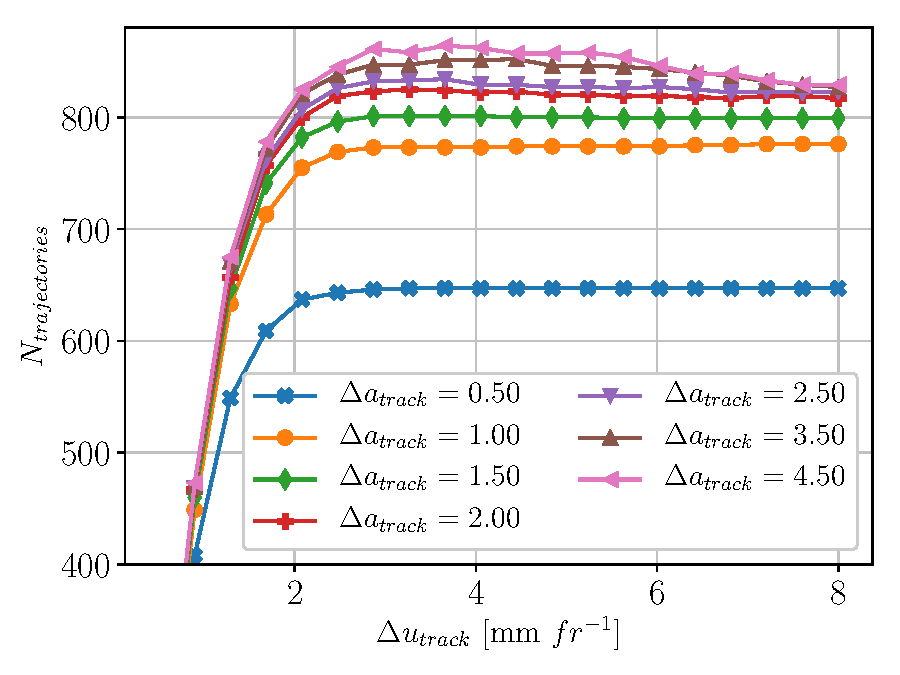
\includegraphics[width=0.65\textwidth]{Num_tracking.pdf}};
\node (a) at (-3.1, 2.9) {\Large{(a)}};

\node[inner sep=0pt] (Len) at (0,-7)
{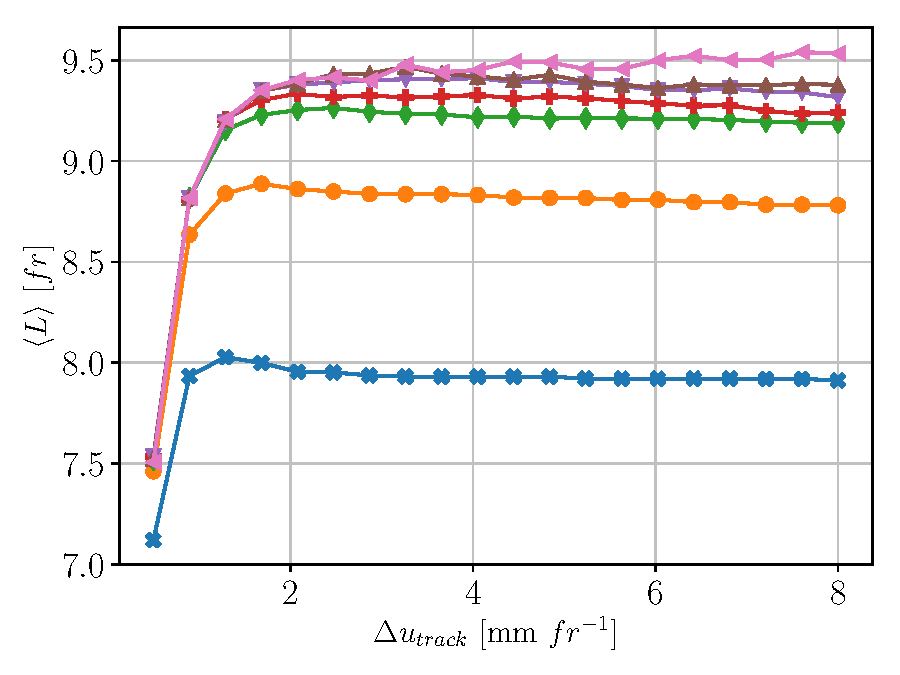
\includegraphics[width=0.65\textwidth]{length_tracking.pdf}};
\node (b) at (-3.1, -4.1) {\Large{(b)}};

\node[inner sep=0pt] (Len) at (0,-14)
{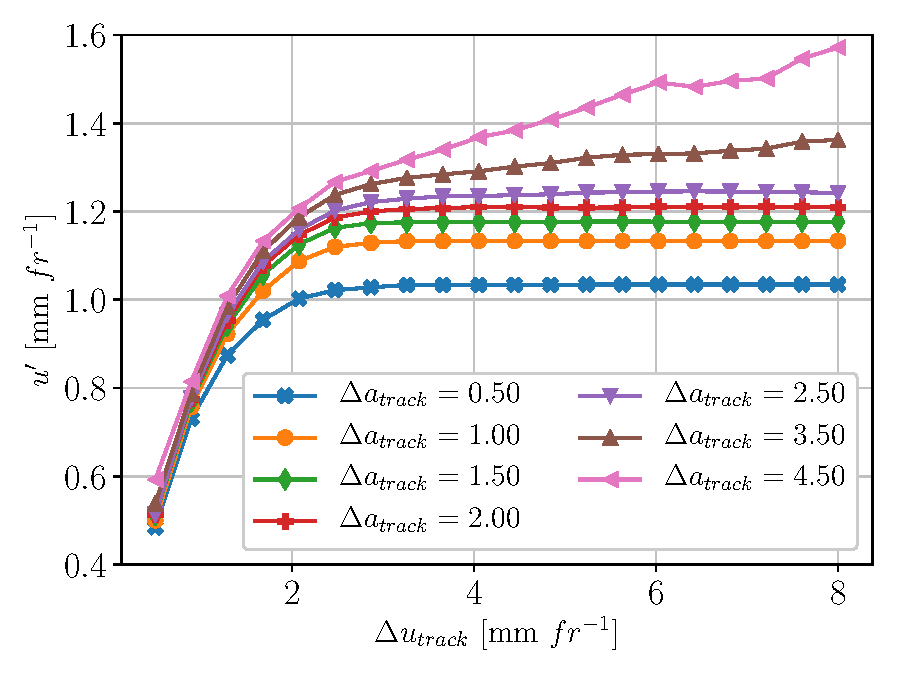
\includegraphics[width=0.65\textwidth]{u_stdv_tracking.pdf}};
\node (c) at (-3.1, -11.1) {\Large{(c)}};

\end{tikzpicture}
	\caption{(a) - Number of found trajectories, (b) - average length of trajectories, and (c) - Root mean square of the calculated velocity. Plotted as a function of the threshold change of velocity, $\Delta u_{\mathrm{track}}$, and acceleration, $\Delta a_{\mathrm{track}}$, per frame \label{fig:tracking_params}}
\end{figure}

